\baselineskip=8mm
\numberwithin{equation}{chapter}
\numberwithin{equation}{section}
\renewcommand{\thesubsection}{\arabic{subsection}.}
\renewcommand{\theequation}{\thesection.\arabic{equation}}
\renewcommand{\thesection}{}
\renewcommand{\thesubsubsection}{\thesubsection\arabic{subsubsection}.}



\vspace{1cm}

\begin{figure}[h]
    \centering
    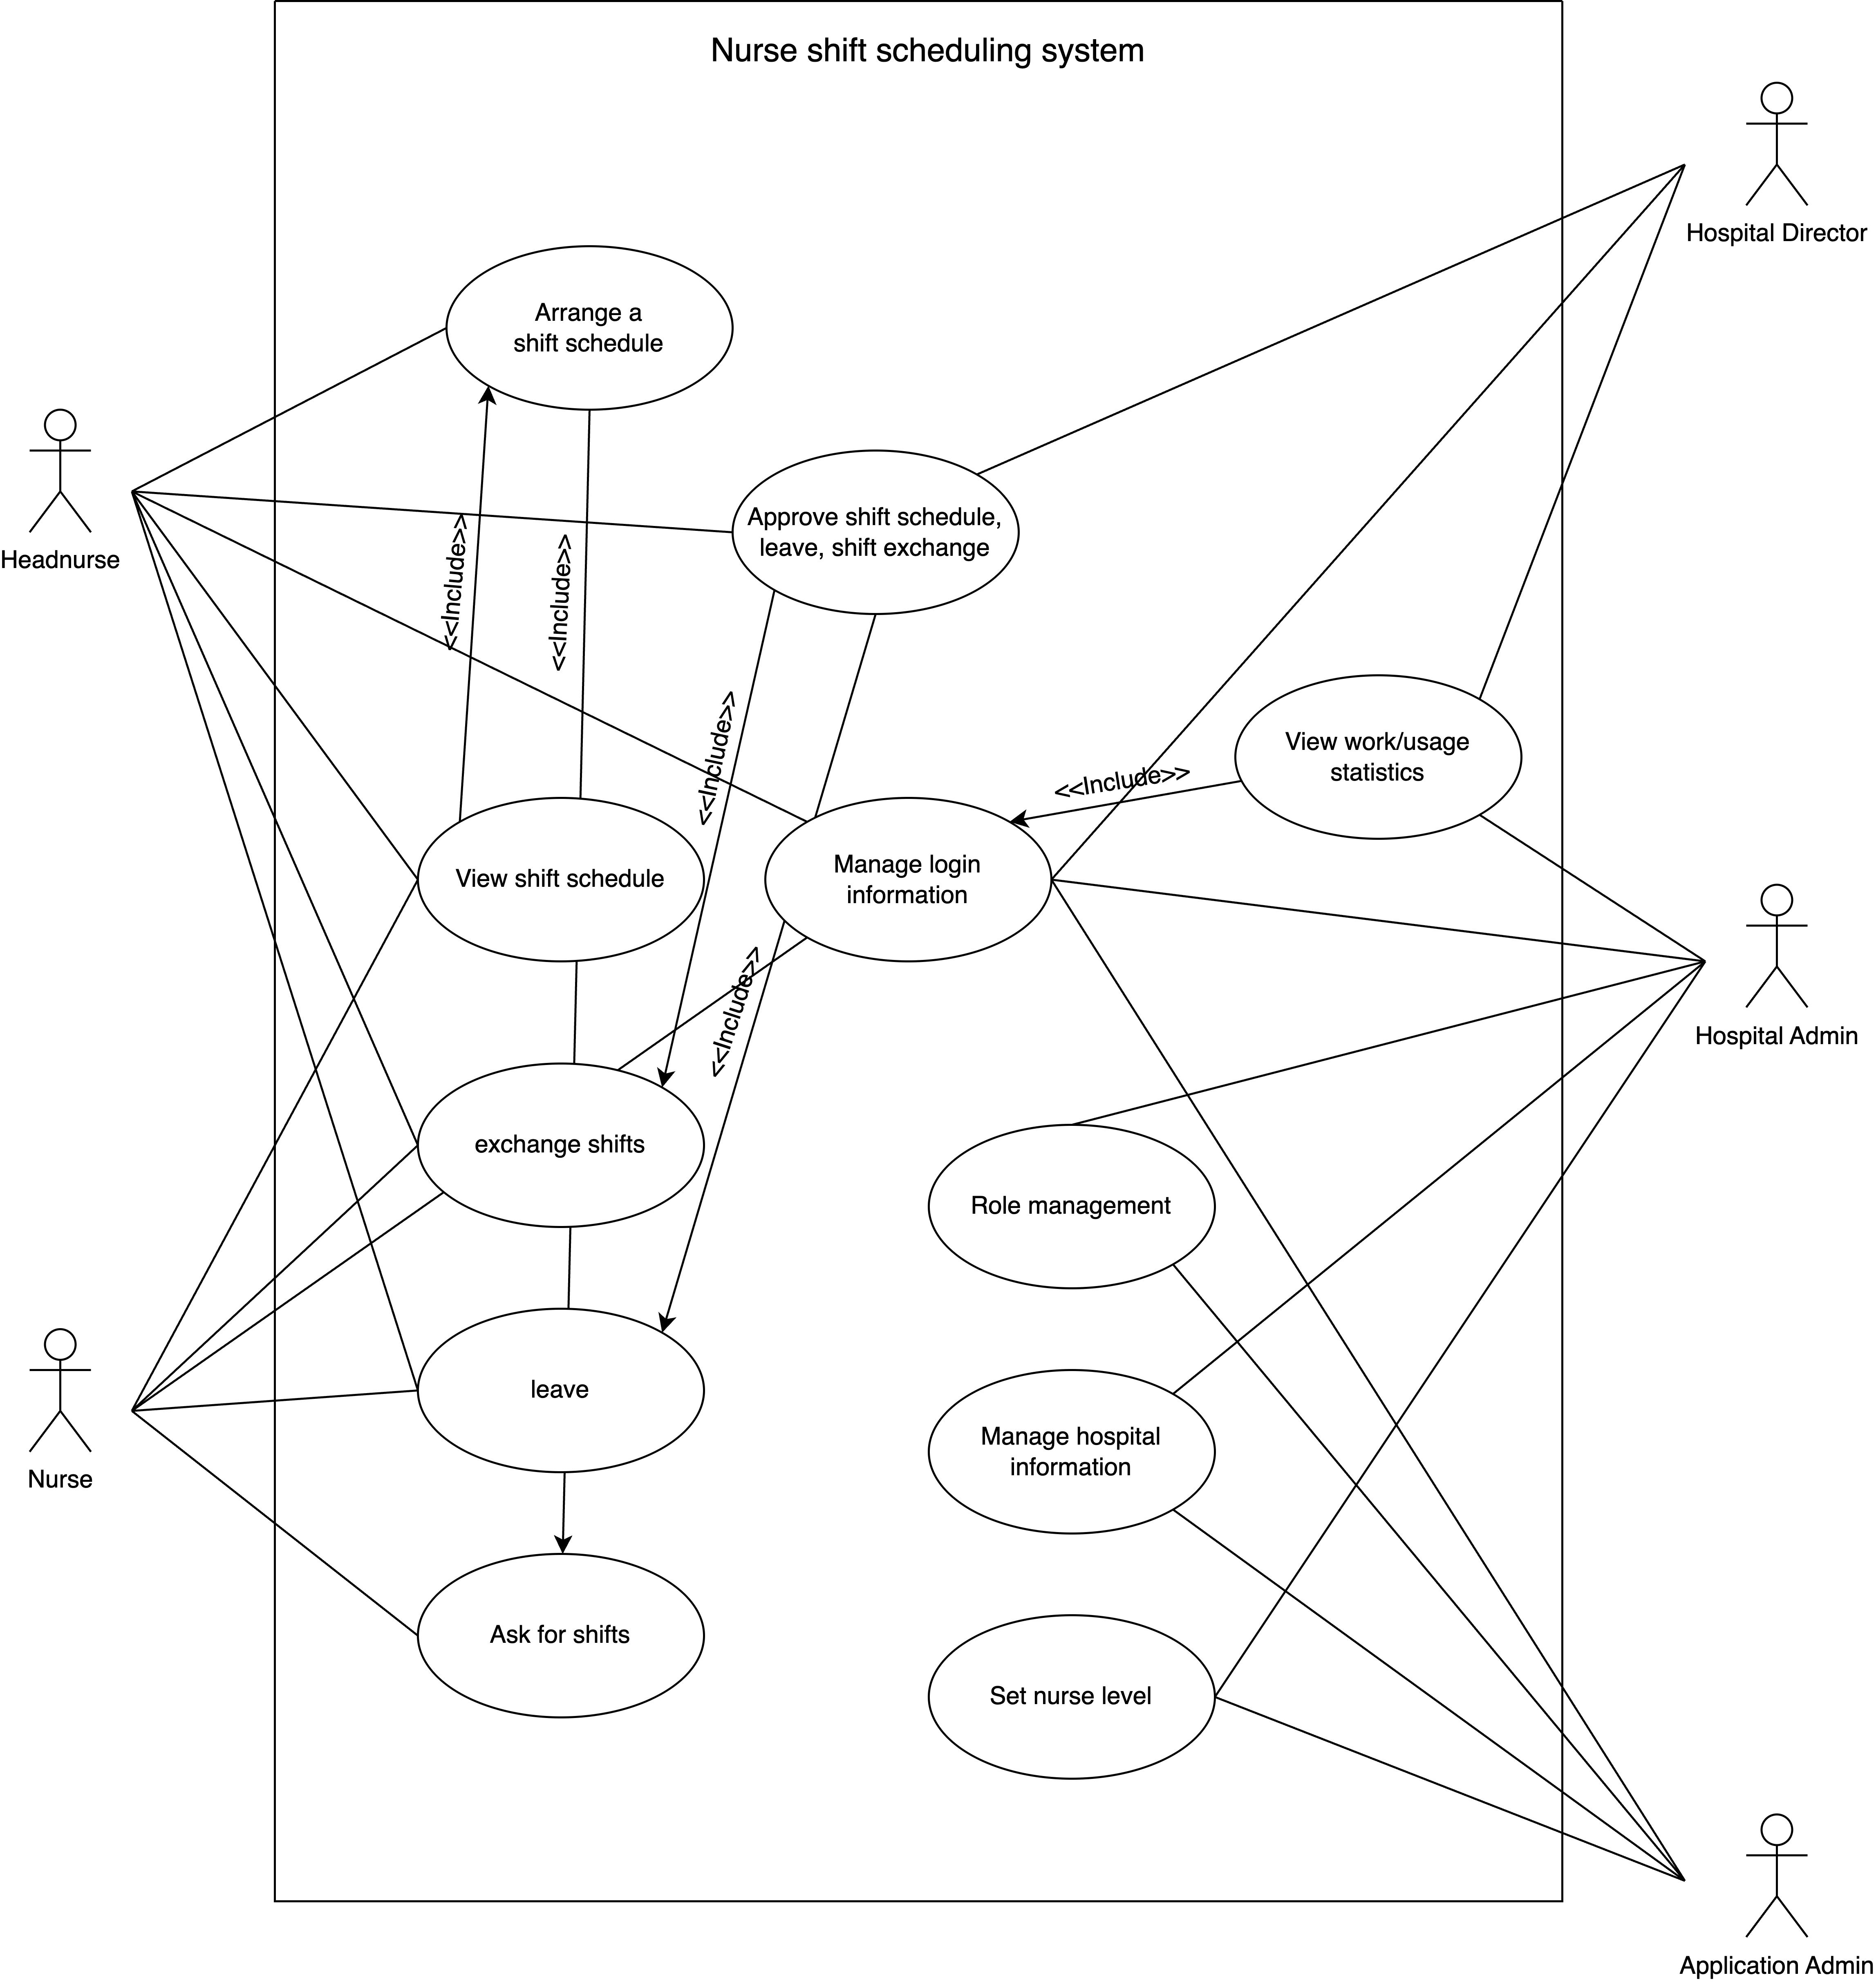
\includegraphics[width=1\textwidth]{UseCase.png}
    \caption{Use Case Diagram}
    \end{figure}
\clearpage


\section{Use Case Description}

\vspace{1cm}

\begin{table}[h]
    \captionsetup{justification=raggedright,singlelinecheck=false}
    \fontsize{10}{18}\selectfont	
    \resizebox{\textwidth}{!}{%
    \centering
    \begin{tabular}{lp{10cm} l} 
        \toprule
        Use Case Title : & Manage login information  & Use Case ID : 1\\ 
        Primary Actor : & Hospital Admin , Hospital Director , Headnurse , Nurse \\ 
        Stakeholder Actor : & Application Admin \\ 
        Main Flow : & ผู้ใช้กรอก Username และ Password ในหน้าเข้าสู่ระบบ ระบบจะทำการตรวจสอบข้อมูลผู้ใช้แล้วก็จะเข้าสู่ตัวระบบและผู้ใช้สามารถออกจากระบบได้ \\ 
        Exception Flow 1 : &  กรณีที่ผู้ใช้กรอก Username หรือ Password ผิดระบบจะให้กรอกใหม่และแสดงสัญลักษณ์ว่าเข้าสู่ระบบไม่สำเร็จ \\ 
        Exception Flow 2 : &  กรณีที่ผู้ใช้ลืม Password ให้ทำการแจ้งผู้ดูแลระบบเพื่อ Reset รหัสผ่าน\\ 
        Exception Flow 3 : &  กรณีที่ผู้ใช้ไม่มีบัญชีต้องทำการติดต่อเจ้าหน้าที่ดูแลระบบ\\ \toprule    
    \end{tabular}
        \caption{Use Case 1: Manage login information}
    }
\end{table}


\begin{table}[h]
    \captionsetup{justification=raggedright,singlelinecheck=false}
    \fontsize{10}{18}\selectfont	
    \resizebox{\textwidth}{!}{%
    \centering
    \begin{tabular}{lp{10cm} l} 
        \toprule
        Use Case Title : & Ask for shifts  & Use Case ID : 2\\ 
        Primary Actor : & Nurse \\
        Stakeholder Actor : & - \\ 
        Main Flow : & พยาบาลสามารถขอเวรได้ในหน้าขอเวร พยาบาลต้องกรอกข้อมูลเวรที่ต้องการจะขอในเดือนถัดไป โดยสามารถดุการขอของพยาบาลคนอื่นได้ หลังจากกรอกข้อมูลขอเวรแล้ว ระบบจะทำการบันทึกลงฐานข้อมูล หลักการจากนั้นหากพยาบาลต้องการแก้ไขเวรที่ขอก็สามารถแก้ไขในหน้าขอเวรได้และสามารถลบเวรที่ขอมาก่อนได้ \\ 
        Exception Flow 1 : &  กรณีที่พยาบาลไม่ได้กรอกข้อมูลขอเวรในบางวัน ระบบจะทำการเซตให้เป็นค่าว่าง \\ 
        Exception Flow 2 : &  กรณีทีี่ระบบปิดการขอเวรไปแล้ว พยาบาลต้องติดต่อกับหัวหน้าพยาบาลในการจัดตารางเวรเอง\\ \toprule 
    \end{tabular}
        \caption{Use Case 2: Ask for shifts}
    }
\end{table}


\begin{table}[h]
    \captionsetup{justification=raggedright,singlelinecheck=false}
    \fontsize{12}{20}\selectfont	
    \resizebox{\textwidth}{!}{%
    \centering
    \begin{tabular}{lp{10cm} l} 
        \toprule
        Use Case Title : & Arrange a shift schedule  & Use Case ID : 3\\ 
        Primary Actor : & Headnurse \\ 
        Stakeholder Actor : & - \\ 
        Main Flow : & หัวหน้าพยาบาลสามารถจัดตารางเวรได้ โดยมีข้อมูลประกอบการตัดสินใจคือการขอเวรของพยาบาล และ ประวัติการทำงานของพยาบาลรายบุคคล หัวหน้าพยาบาลสามารถดูระดับของพยาบาลได้ หลังจากการจัดตารางเสร็จแล้วหัวหน้าพยาบาลสามารถแก้ไขตารางนั้นได้ สามารถลบได้ หากหัวหน้าพยาบาลคิดว่าเหมาะสมแล้วก็สามารถส่งเรื่องไปยังผู้อำนวยการโรงพยาบาลเพื่ออนุมัติการใช้งานตารางเวรได้ \\ 
        Exception Flow 1 : &  กรณีที่หัวหน้าพยาบาลยื่นเรื่องไปที่ผู้อำนวยการโรงพยาบาลแล้ว ต้องการแก้ไขตารางใหม่ ต้องส่งให้ผู้อำนวยการอีกรอบเพื่อยืนยัน \\ 
        Exception Flow 2 : &  กรณีที่ตารางเวรอนุมัติใช้จากผู้อำนวยการโรงพยาบาลแล้ว หากมีความประสงค์ที่จะแก้ไขตารางให้เป็นการแลกเวรแทน\\ \toprule
    \end{tabular}
        \caption{Use Case 3: Arrange a shift schedule}
    }
\end{table}


\begin{table}
    \captionsetup{justification=raggedright,singlelinecheck=false}
    \fontsize{12}{20}\selectfont	
    \resizebox{\textwidth}{!}{%
    \centering
    \begin{tabular}{lp{10cm} l} 
        \toprule
        Use Case Title : & Approve shift schedule, leave, shift exchange  & Use Case ID : 4\\ 
        Primary Actor : & Headnurse , Hospital Director \\ 
        Stakeholder Actor : & - \\ 
        Main Flow : & หัวหน้าพยาบาลและผู้อำนวยการโรงพยาบาลสามารถอนุมัติเรื่องต่างๆได้ โดยมีการกำหนดให้ผู้อำนวยการโรงพยาบาลสามารถอนุมัติตารางเวรและการลา หัวหน้าพยาบาลสามารถอนุมัติการลาและการแลกเวรของพยาบาลได้ โดยการกดยืนยันการลา หัวหน้าพยาบาลต้องยืนยันก่อนที่จะส่งเรื่องไปยังผู้อำนวยการ หากกดยืนยันแล้วจะไม่สามารถยกเลิกได้ หากไม่ยืนยันตัวระบบจะมีข้อมูลรายละเอียดให้กรอกเพื่อบอกเหตุผล \\ 
        Exception Flow 1 : &  กรณีการลาหากหัวหน้าพยาบาลยืนยันไปแล้วแต่ผู้อำนวยการโรงพยาบาลไม่ยืนยันจะถือเป็นการลาที่ไม่สำเร็จ พยาบาลต้องยื่นเรื่องเข้ามาในระบบใหม่\\ 
        Exception Flow 2 : &  กรณีที่หัวหน้าพยาบาลไม่ได้ยืนยัน ผู้อำนวยการจะไม่สามารถยืนยันได้ ต้องผ่านหัวหน้าพยาบาลก่อน\\ \toprule
    \end{tabular}
        \caption{Use Case 4: Approve shift schedule, leave, shift exchange}
    }
\end{table}


\begin{table}
    \captionsetup{justification=raggedright,singlelinecheck=false}
    \fontsize{12}{20}\selectfont	
    \resizebox{\textwidth}{!}{%
    \centering
    \begin{tabular}{lp{10cm} l} 
        \toprule
        Use Case Title : & View shift schedule  & Use Case ID : 5\\ 
        Primary Actor : & Headnurse , Nurse \\ 
        Stakeholder Actor : & - \\ 
        Main Flow : & หัวหน้าพยาบาลและพยาบาลสามารถดูตารางเวรของตัวเองได้ในตารางเวร ระบบจะแสดงข้อมูลการคำนวณต่างๆและตารางเวร หัวหน้าพยาบาลและพยาบาลสามารถเปลี่ยนรูปแบบของหน้าการแสดงผลได้ \\ 
        Exception Flow 1 : &  หากขึ้นเดือนใหม่และยังจัดตารางเวรไม่เสร็จระบบจะขึ้นตารางของเดือนก่อนให้\\ 
        \toprule
    \end{tabular}
        \caption{Use Case 5: View shift schedule}
    }
\end{table}


\begin{table}
    \captionsetup{justification=raggedright,singlelinecheck=false}
    \fontsize{12}{20}\selectfont	
    \resizebox{\textwidth}{!}{%
    \centering
    \begin{tabular}{lp{10cm} l} 
        \toprule
        Use Case Title : & Exchange shifts  & Use Case ID : 6\\ 
        Primary Actor : & Headnurse , Nurse \\ 
        Stakeholder Actor : & - \\ 
        Main Flow : & หัวหน้าพยาบาลสามารถแลกเวรกันได้หลังจากการจัดตารางเวร การแลกเวรจะแลกเวรได้โดยมีเงื่อนไขคือระดับของพยาบาลต้องมีจำนวนถึงกำหนดในวันที่แลก การแลกเวรเมื่อแลกแล้วจะต้องทำงานติดต่อกันไม่เกิน 20 ชั่วโมง  โดยสามารถแก้ไขการขอแลกเวรและลบคำขอแลกเวรได้ การขอแลกพยาบาลทั้งสองต้องสร้างการแลกเวรในระบบและกดยืนยันทั้งสอง เรื่องจะส่งไปแจ้งเตือนให้หัวหน้าพยาบาบทราบ หลังจากนั้นหัวหน้าพยาบาลจะเป็นคนตัดสินใจในการแลกเวร หากยืนยันแล้วการแลกเวรถือเป็นอันเสร็จสิ้น\\ 
        Exception Flow 1 : &  กรณีที่ต้องการแก้ไขหรือยกเลิกหลังจากการยืนยันของหัวหน้าพยาบาลจะไม่สามารถทำได้ ถ้าหากต้องการทำรายการใหม่ต้องทำการแลกเวรใหม่ตั้งแต่ต้นเท่านั้น\\ 
        \toprule
    \end{tabular}
        \caption{Use Case 6: Exchange shifts}
    }
\end{table}


\begin{table}
    \captionsetup{justification=raggedright,singlelinecheck=false}
    \fontsize{12}{20}\selectfont	
    \resizebox{\textwidth}{!}{%
    \centering
    \begin{tabular}{lp{10cm} l} 
        \toprule
        Use Case Title : & leave  & Use Case ID : 7\\ 
        Primary Actor : & Headnurse , Nurse \\ 
        Stakeholder Actor : & - \\ 
        Main Flow : & หัวหน้าพยาบาลและพยาบาลสามารถขอลาได้ หากต้องการขอลาสามารถเข้าเมนูลาและกรอกข้อมูลการลา และส่งการลาให้หัวหน้าพยาบาลยืนยันและรอให้ผู้อำนวยการยืนยัน\\ 
        Exception Flow 1 : &  กรณีที่กรอกลาแล้ว อยากยกเลิกการลาหรือแก้ไขการลาของตนเอง สามารถแก้ไขและลบได้ก่อนการยืนยันของหัวหน้าพยาบาล\\  
        \toprule
    \end{tabular}
        \caption{Use Case 7: leave}
    }
\end{table}
    

\begin{table}
    \captionsetup{justification=raggedright,singlelinecheck=false}
    \fontsize{12}{20}\selectfont	
    \resizebox{\textwidth}{!}{%
    \centering
    \begin{tabular}{lp{10cm} l} 
        \toprule
        Use Case Title : & Role management  & Use Case ID : 8\\ 
        Primary Actor : & Application Admin , Hospital Admin \\ 
        Stakeholder Actor : & - \\ 
        Main Flow : & แอดมินสามารถจัดการสิทธิ์ของผู้ใช้งานได้ โดยสามารถเพิ่มสิทธ์ ลบสิทธิ์ แก้ไขสิทธิ์และสามารถกำหนดสิทธิ์ให้ผู้ใช้ในระบบผ่านทางเมนู\\ 
        Exception Flow 1 : &  หากแอดมินลบสิทธิ์ไปแล้วผู้ใช้เป็นสิทธิ์นั้น ระบบจะกำหนดสิทธิ์เป็นค่าว่าง และแจ้งเตือนให้แอดมินทราบ \\ 
        \toprule
    \end{tabular}
        \caption{Use Case 8: Role management}
    }
\end{table}


\begin{table}
    \captionsetup{justification=raggedright,singlelinecheck=false}
    \fontsize{12}{20}\selectfont	
    \resizebox{\textwidth}{!}{%
    \centering
    \begin{tabular}{lp{10cm} l} 
        \toprule
        Use Case Title : & Manage hospital information  & Use Case ID : 9\\ 
        Primary Actor : & Application Admin , Hospital Admin \\ 
        Stakeholder Actor : & - \\ 
        Main Flow : & แอดมินสามารถจัดการข้อมูลของโรงพยาบาลโดยเข้าถึงผ่านเมนู หากต้องการเพิ่มโรงพยาบาลสามารถทำได้โดยกรอกข้อมูลของโรงพยาบาล หากทำการกรอกแล้วก็บันทึก ระบบจะบันทึกลงฐานข้อมูลและแสดงบนหน้าจอว่าบันทึกเสร็จสิ้น\\ 
        Exception Flow 1 : & กรณีที่แอดมินต้องการแก้ไขโรงพยาบาลหรือลบสามารถทำได้โดยการกดปุ่มบนเมนูของหน้าจัดการข้อมูลโรงพยาบาล \\ 
        \toprule
    \end{tabular}
        \caption{Use Case 9: Manage hospital information}
    }
\end{table}

\begin{table}
    \captionsetup{justification=raggedright,singlelinecheck=false}
    \fontsize{12}{20}\selectfont	
    \resizebox{\textwidth}{!}{%
    \centering
    \begin{tabular}{lp{10cm} l} 
        \toprule
        Use Case Title : & Set nurse level  & Use Case ID : 10\\ 
        Primary Actor : & Application Admin , Hospital Admin \\ 
        Stakeholder Actor : & - \\ 
        Main Flow : & แอดมินสามารถจัดการข้อมูลระดับของพยาบาลโดยการเข้าเมนูระดับของพยาบาล และทำการกรอกข้อมูลของระดับพยาบาล กำหนดระดับของพยาบาลกับพยาบาล \\ 
        Exception Flow 1 : &  แอดมินสามารถจัดการข้อมูลระดับของพยาบาบลโดยเข้าถึงผ่านเมนู หากต้องการเพิ่มระดับของพยาบาล สามารถทำได้โดยกรอกข้อมูลชื่อ ระดับ หากทำการกรอกแล้วก็บันทึก ระบบจะบันทึกลงฐานข้อมูลและแสดงบนหน้าจอว่าบันทึกเสร็จสิ้น \\ 
        \toprule
    \end{tabular}
        \caption{Use Case 10: Set nurse level}
    }
\end{table}
    


\begin{table}
    \captionsetup{justification=raggedright,singlelinecheck=false}
    \fontsize{12}{20}\selectfont	
    \resizebox{\textwidth}{!}{%
    \centering
    \begin{tabular}{lp{10cm} l} 
        \toprule
        Use Case Title : & View work/usage statistics  & Use Case ID : 11\\ 
        Primary Actor : & Hospital Admin , Hospital Director \\ 
        Stakeholder Actor : & - \\ 
        Main Flow : & แอดมินของโรงพยาบาลและผู้อำนวยการโรงพยาบาลสามารถดูสถิติการใช้งานของพยาบาลได้ สามารถเข้าถึผ่านทางเมนูดูสถิติการทำงาน สามารถเลือก ช่วงเวลาของวัน การทำงานของเดือน และอื่นๆเ \\ 
        Exception Flow 1 : &  กรณีที่ไม่พบข้อมูลระบบจะแสดงผลให้แอดมินหรือผู้อำนวยการทราบ \\ 
        \toprule
    \end{tabular}
        \caption{Use Case 11: View work/usage statistics}
    }
\end{table}

    